\documentclass[pdflatex,compress]{beamer}

%\usetheme[dark,framenumber,totalframenumber]{ElektroITK}
\usetheme[darktitle,framenumber,totalframenumber]{ElektroITK}
\usepackage{graphicx}
\usepackage{multicol}

\title{Data Communications}
\subtitle{Chapter 2 - Protocol Architecture}

\author{Mifta Nur Farid, M.T.}

\begin{document}

\maketitle

\begin{frame}
	\frametitle{The Need for a Protocol Architecture}
	To transfer data several tasks must be performed:
	\begin{enumerate}
		\item The source must either activate the direct communications path or inform the network of the identity of the desired destination system
		\item The source system must ascertain that the destination system is prepared to receive data
		\item The file transfer application on the source system must ascertain that the file management program on the destination system is prepared to accept and store the file for this particular user
		\item A format translation function may need to be performed by one or the other system if the file formats used on the two systems are different
	\end{enumerate}
\end{frame}

\begin{frame}
	\frametitle{Functions of Protocol Architecture}
	\begin{itemize}
		\item Breaks logic into subtask modules which are implemented separately
		\item Modules are arranged in a vertical stack
		\begin{itemize}
			\item Each layer in the stack performs a subset of functions
			\item Relies on next lower layer for primitive functions
			\item Provides services to the next higher layer
			\item Changes in one layer should not require changes in other layers
		\end{itemize}
	\end{itemize}
\end{frame}

\begin{frame}
	\frametitle{Key Features of a Protocol}
	\begin{itemize}
		\item A protocol is a set of rules or conventions that allow peer layers to communicate
		\item The key features of a protocol are:
		\begin{itemize}
			\item \textbf{Syntax}\\
			Format of data blocks
			\item \textbf{Semantics}\\
			Control information for coordination and error handling
			\item \textbf{Timing}\\
			Speed matching and sequencing
		\end{itemize}
	\end{itemize}
\end{frame}

\begin{frame}
	\frametitle{A Simple Protocol Architecture}
	\begin{enumerate}
		\item Agents involved:
		\begin{itemize}
			\item Applications
			\item Computers
			\item Networks
		\end{itemize}
		\item Examples of applications include file transfer and electronic mail
		\item These execute on computers that support multiple simultaneous applications
	\end{enumerate}
\end{frame}

\begin{frame}
	\frametitle{Communication Layers}
	\begin{itemize}
		\item Communication tasks are organized into three relatively independent layers:
		\begin{enumerate}
			\item \textbf{Network access layer}\\
			Concerned with the exchange of data between a computer and the network to which it is attached
			\item \textbf{Transport layer}\\
			Collects mechanisms in a common layer shared by all applications
			\item \textbf{Application layer}\\
			Contains logic to support applications
		\end{enumerate}
	\end{itemize}
\end{frame}

\begin{frame}
	\begin{center}
		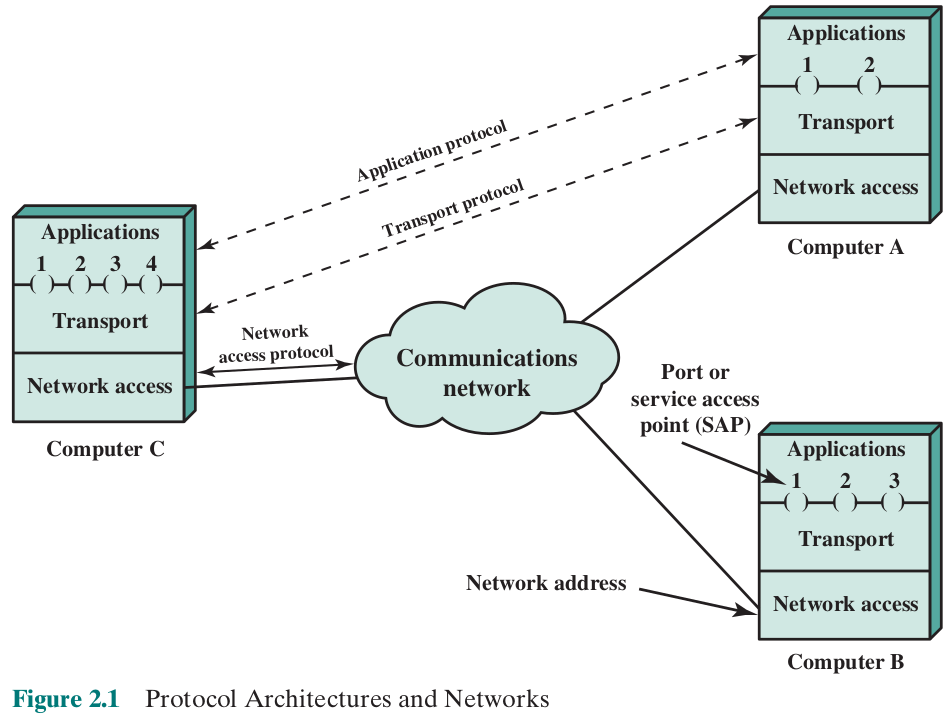
\includegraphics[width=0.8\linewidth]{img/img01}
	\end{center}
\end{frame}

\begin{frame}
	\begin{center}
		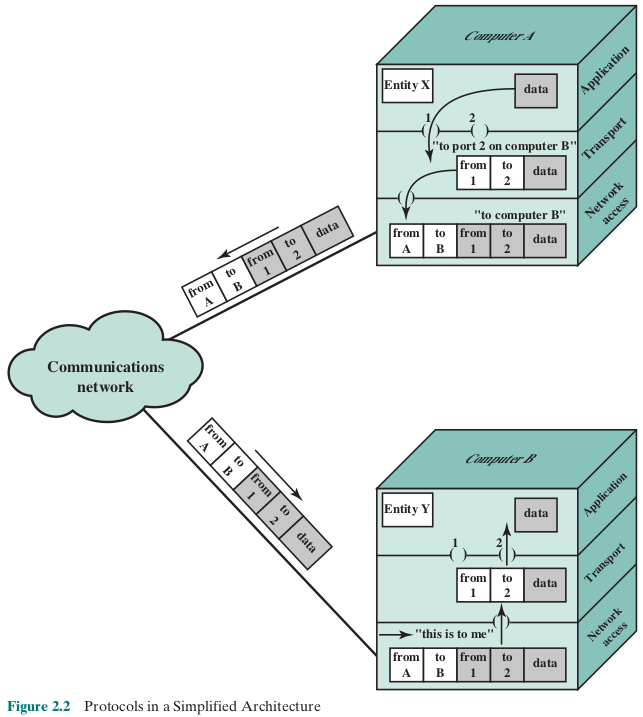
\includegraphics[height=0.9\textheight]{img/img02}
	\end{center}
\end{frame}

\begin{frame}
	\frametitle{TCP/IP Protocol Architecture}
	\begin{itemize}
		\item Result of protocol research and development conducted on ARPANET
		\item Referred to as TCP/IP protocol suite
		\item TCP/IP comprises a large collection of protocols that are Internet standards
	\end{itemize}
\end{frame}

\begin{frame}
	\begin{center}
		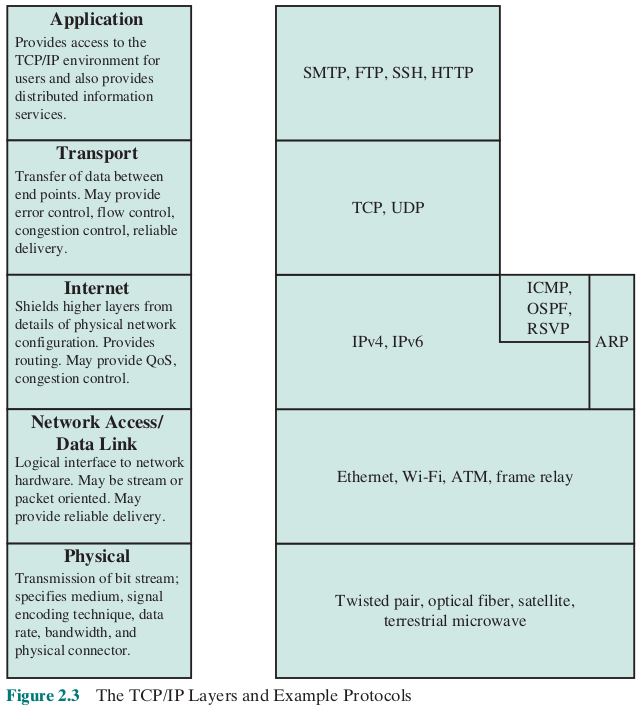
\includegraphics[height=0.9\textheight]{img/img03}
	\end{center}
\end{frame}

\begin{frame}
	\frametitle{Physical Layer}
	\begin{itemize}
		\item Covers the physical interface between computer and network
		\item Concerned with issues like:
		\begin{itemize}
			\item Characteristics of transmission medium
			\item Nature of the signals
			\item Data rates
		\end{itemize}
	\end{itemize}
\end{frame}

\begin{frame}
	\frametitle{Network Access/Data Link Layer}
	\begin{itemize}
		\item Covers the exchange of data between an end system and the network that it is attached to
		\item Concerned with:
		\begin{itemize}
			\item Access to and routing data across a network for two end systems attached to the same network
		\end{itemize}
	\end{itemize}
\end{frame}

\begin{frame}
	\frametitle{Internet Layer}
	\begin{itemize}
		\item Implements procedures needed to allow data to travel across multiple interconnected networks
		\item Uses the Internet Protocol (IP) to provide routing function
		\item Implemented in end systems and routers
	\end{itemize}
\end{frame}

\begin{frame}
	\frametitle{Host-to-Host (Transport) Layer}
	\begin{itemize}
		\item May provide reliable end-to-end service or merely an end-to-end delivery service without reliability mechanisms
		\item \textbf{Transmission Control Protocol (TCP)}\\
		Most commonly used protocol to provide this functionality
	\end{itemize}
\end{frame}

\begin{frame}
	\frametitle{Application Layer}
	\begin{itemize}
		\item Contains the logic needed to support the various user applications
		\item A separate module is needed for each different type of application that is peculiar to that application
	\end{itemize}
\end{frame}

\begin{frame}
	\begin{center}
		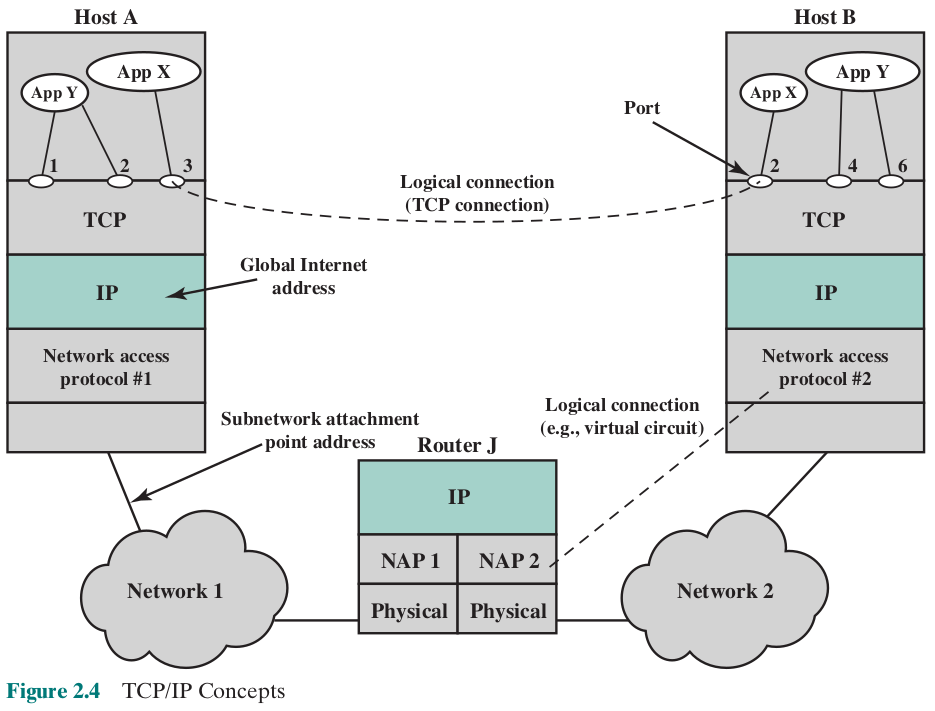
\includegraphics[height=0.9\textheight]{img/img04}
	\end{center}
\end{frame}

\begin{frame}
	\frametitle{TCP/IP Address Requirements}
	\begin{itemize}
		\item Two levels of addressing are needed:
		\begin{itemize}
			\item Each host on a subnetwork must have a unique global internet address
			\item Each process with a host must have an address (known as a port) that is unique within the host
		\end{itemize}
	\end{itemize}
\end{frame}

\begin{frame}
	\begin{center}
		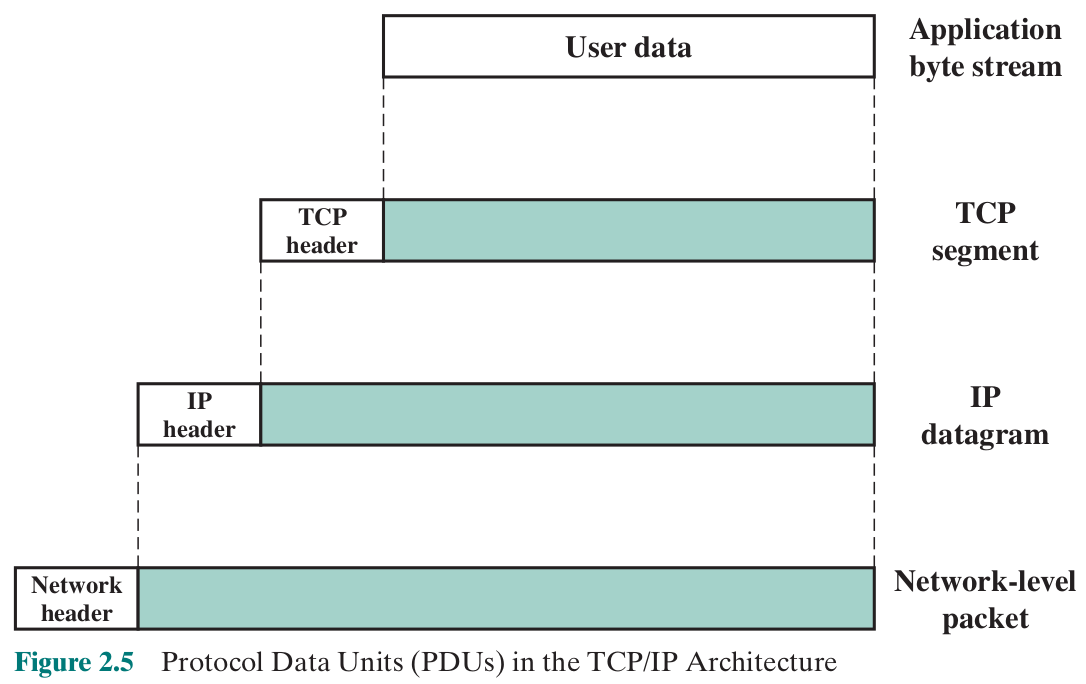
\includegraphics[height=0.8\textheight]{img/img05}
	\end{center}
\end{frame}

\begin{frame}
	\frametitle{Transmission Control Protocol (TCP)}
	\begin{itemize}
		\item TCP is the transport layer protocol for most applications
		\item TCP provides a reliable connection for transfer of data between applications
		\item A TCP segment is the basic protocol unit
		\item TCP tracks segments between entities for duration of each connection
	\end{itemize}
\end{frame}

\begin{frame}
	\begin{center}
		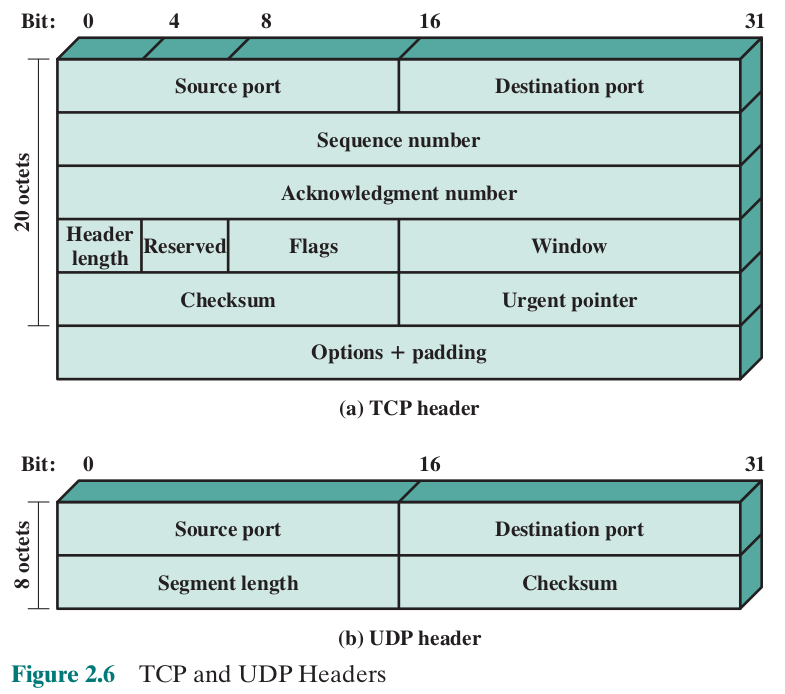
\includegraphics[height=0.9\textheight]{img/img06}
	\end{center}
\end{frame}

\begin{frame}
	\frametitle{User Datagram Protocol (UDP)}
	\begin{itemize}
		\item Alternative to TCP
		\item Does not guarantee delivery, preservation of sequence, or protection against duplication
		\item Enables a procedure to send messages to other procedures with a minimum of protocol mechanism
		\item Adds port addressing capability to IP
		\item Used with Simple Network Management Protocol (SNMP)
		\item Includes a checksum to verify that no error occurs in the data
	\end{itemize}
\end{frame}

\begin{frame}
	\begin{center}
		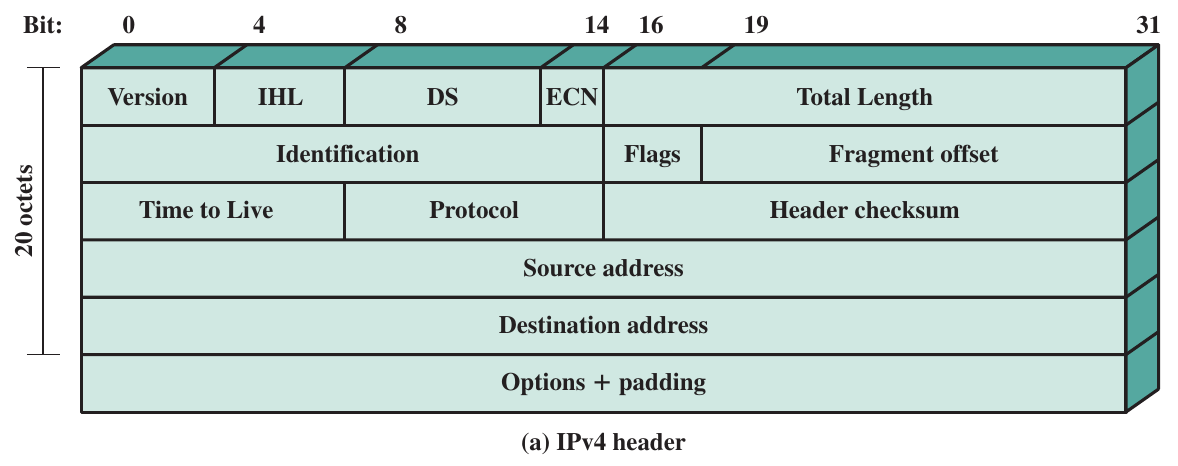
\includegraphics[width=\linewidth]{img/img07}
	\end{center}
\end{frame}

\begin{frame}
	\begin{center}
		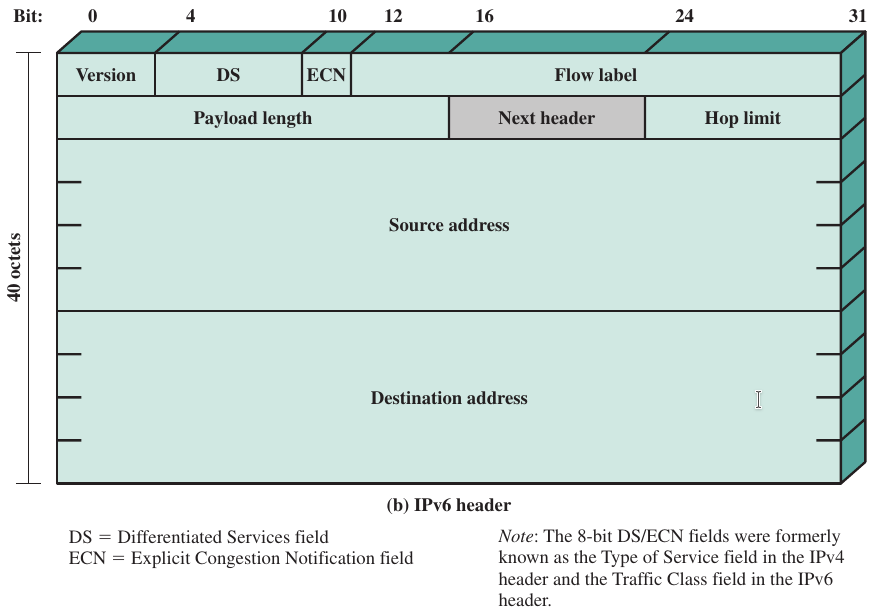
\includegraphics[width=0.8\linewidth]{img/img08}
	\end{center}
\end{frame}

\begin{frame}
	\begin{center}
		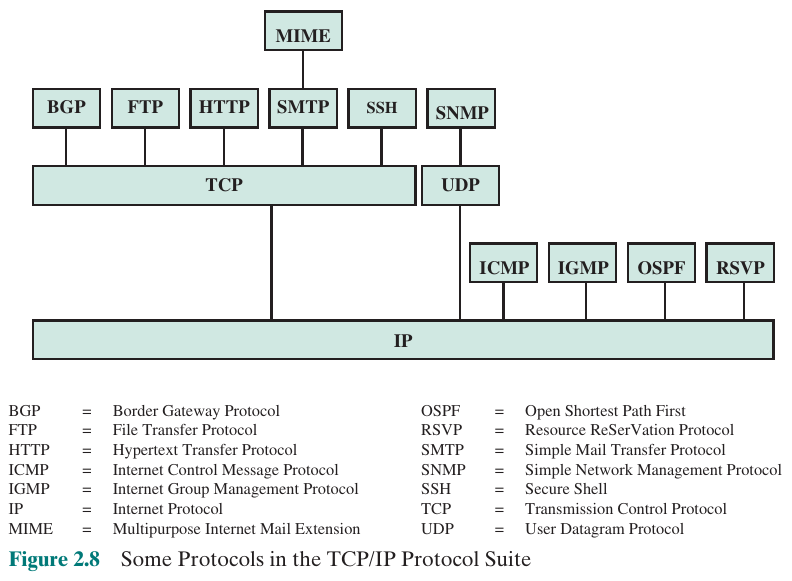
\includegraphics[height=0.9\textheight]{img/img09}
	\end{center}
\end{frame}

\begin{frame}
	\frametitle{Service Primitives and Parameters}
	\begin{itemize}
		\item Services between adjacent layers
		\item Expressed as:
		\begin{itemize}
			\item Primitives
			\begin{itemize}
				\item Specify the function to be performed
			\end{itemize}
			\item Parameters
			\begin{itemize}
				\item Used to pass data and control information
			\end{itemize}
		\end{itemize}
	\end{itemize}
\end{frame}

\begin{frame}
	\begin{center}
		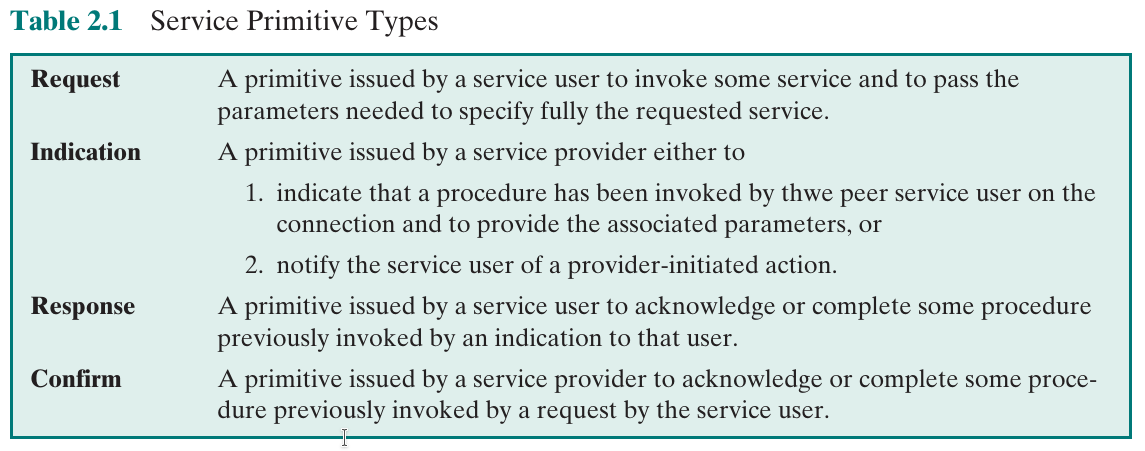
\includegraphics[width=\linewidth]{img/img11}
	\end{center}
\end{frame}

\begin{frame}
	\begin{center}
		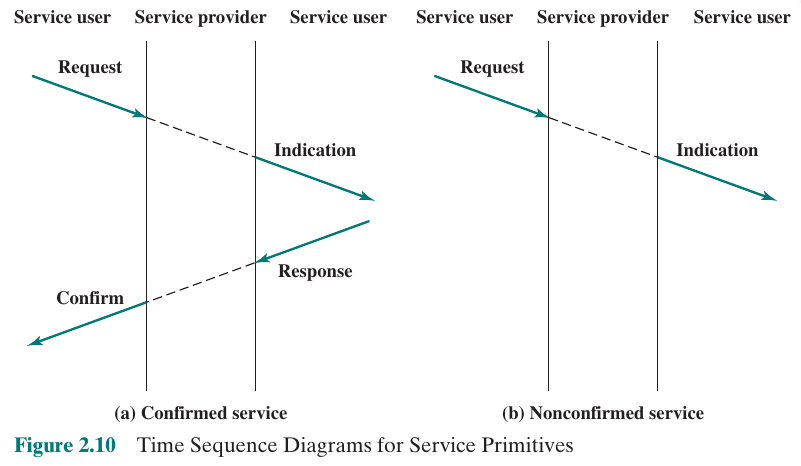
\includegraphics[width=\linewidth]{img/img12}
	\end{center}
\end{frame}

\begin{frame}
	\frametitle{Traditional Internet-Based\\Applications}
	Three common applications that have been standardized to operate on top of TCP are:
	\begin{enumerate}
		\item Simple Mail Transfer Protocol (SMTP)
		\begin{itemize}
			\item Provides a mechanism for transferring messages among separate hosts
		\end{itemize}
		\item File Transfer Protocol (FTP)
		\begin{itemize}
			\item Used to send files from one system to another under user command
			\item Both text and binary files are accommodated
		\end{itemize}
		\item Secure Shell (SSH)
		\begin{itemize}
			\item Provides a secure remote logon capability
		\end{itemize}
	\end{enumerate}
\end{frame}

\begin{frame}
	\begin{center}
		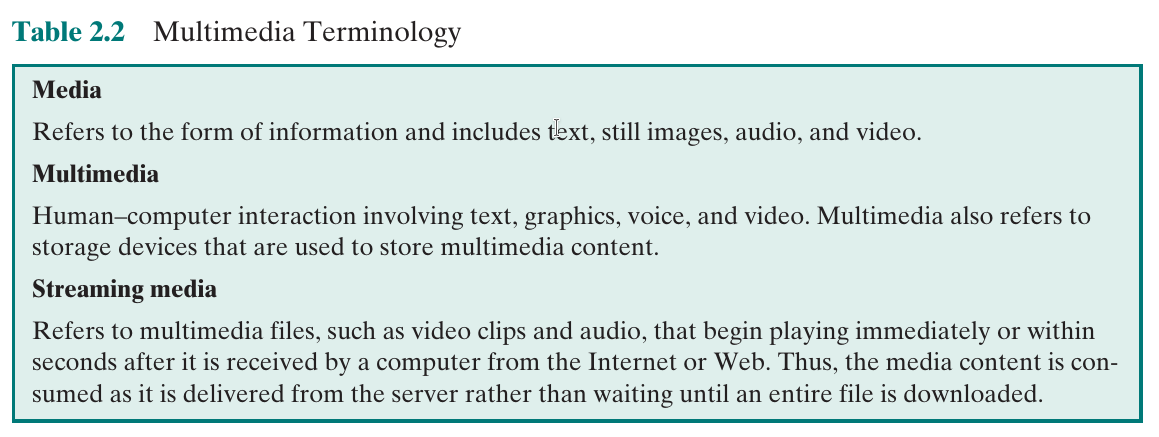
\includegraphics[width=\linewidth]{img/img13}
	\end{center}
\end{frame}

\begin{frame}
	\begin{center}
		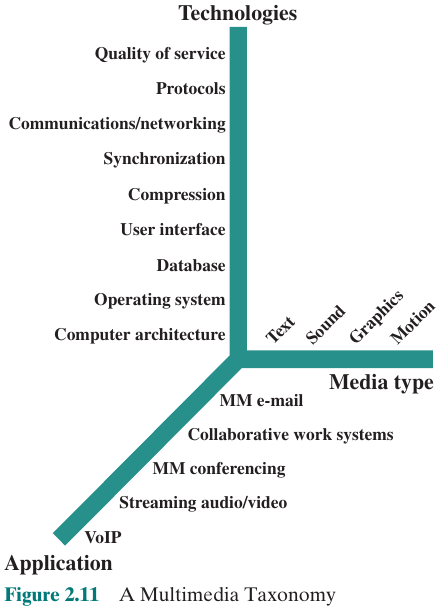
\includegraphics[height=0.9\textheight]{img/img14}
	\end{center}
\end{frame}

\begin{frame}
	\frametitle{Media Types}
	\begin{itemize}
		\item \textbf{audio} generally encompasses sounds that are produced by the human speech mechanism
		\item \textbf{image} supports the communication of individual pictures, charts, or drawings
		\item \textbf{video} service carries sequences of pictures in time
		\item \textbf{text} is information that can be entered via a keyboard and is directly readable and printable
	\end{itemize}
\end{frame}

\begin{frame}
	\begin{center}
		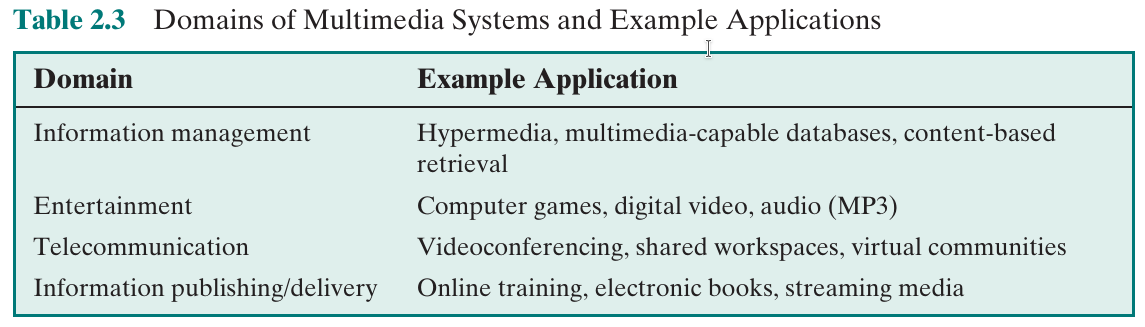
\includegraphics[width=\linewidth]{img/img15}
	\end{center}
\end{frame}

\begin{frame}
	\frametitle{Multimedia Applications}
	\begin{itemize}
		\item Information systems
		\begin{itemize}
			\item[$ \circ $] Information kiosks, electronic books that include audio and video, and multimedia expert systems
		\end{itemize}
		\item Communication systems
		\begin{itemize}
			\item[$ \circ $] Support collaborative work, such as videoconferencing
		\end{itemize}
		\item Entertainment systems
		\begin{itemize}
			\item[$ \circ $] Computer and network games and other forms of audiovisual entertainment
		\end{itemize}
		\item Business systems
		\begin{itemize}
			\item[] Business-oriented multimedia presentations, video brochures, and online shopping
		\end{itemize}
		\item Educational systems
		\begin{itemize}
			\item[$ \circ $] Electronic books with a multimedia component, simulation and modeling applets, and other teaching support systems
		\end{itemize}
	\end{itemize}
\end{frame}

\begin{frame}
	\frametitle{Multimedia Technologies}
	Some technologies that are relevant to the support of multimedia applications are:
	\begin{itemize}
		\item Compression
		\begin{itemize}
			\item[$ \circ $] JPG for still images
			\item[$ \circ $] MPG for video
		\end{itemize}
		\item Communications/networking\begin{itemize}
			\item[$ \circ $] Refers to the transmission and networking technologies that can support high-volume multimedia traffic
		\end{itemize}
		\item Protocols
		\begin{itemize}
			\item[$ \circ $] Real-time Transport Protocol (RTP)
			\item[$ \circ $] Session Initiation Protocol (SIP)
		\end{itemize}
		\item Quality of service (QoS)
		\begin{itemize}
			\item[$ \circ $] Can deal with priority, delay constraints, delay variability constraints, and other similar requirements
		\end{itemize}
	\end{itemize}
\end{frame}

\begin{frame}
	\frametitle{Sockets Programming}
	\begin{itemize}
		\item Concept was developed in the 1980s in the UNIX environment as the Berkeley Sockets Interface
		\begin{itemize}
			\item De facto standard application programming interface (API)
			\item Basis for Window Sockets (WinSock)
		\end{itemize}
		\item Enables communication between a client and server process
		\item May be connection oriented or connectionless
	\end{itemize}
\end{frame}

\begin{frame}
	\frametitle{The Socket}
	\begin{itemize}
		\item Formed by the concatenation of a port value and an IP address
		\begin{itemize}
			\item Unique throughout the Internet
		\end{itemize}
		\item Used to define an API
		\begin{itemize}
			\item Generic communication interface for writing programs that use TCP or UDP
		\end{itemize}
		\item Stream sockets
		\begin{itemize}
			\item All blocks of data sent between a pair of sockets are guaranteed for delivery and arrive in the order that they were sent
		\end{itemize}
		\item Datagram sockets
		\begin{itemize}
			\item Delivery is not guaranteed, nor is order necessarily preserved
		\end{itemize}
		\item Raw sockets
		\begin{itemize}
			\item Allow direct access to lower-layer protocols
		\end{itemize}
	\end{itemize}
\end{frame}

\begin{frame}
	\begin{center}
		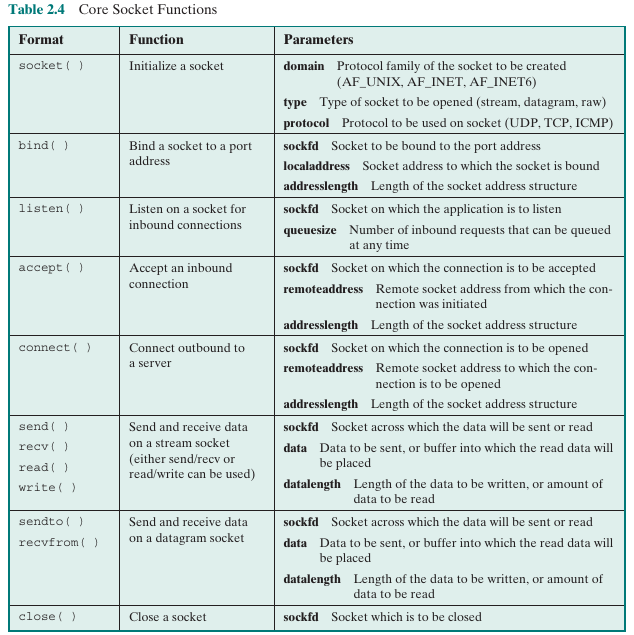
\includegraphics[height=0.8\textheight]{img/img16}
	\end{center}
\end{frame}

\begin{frame}
	\begin{center}
		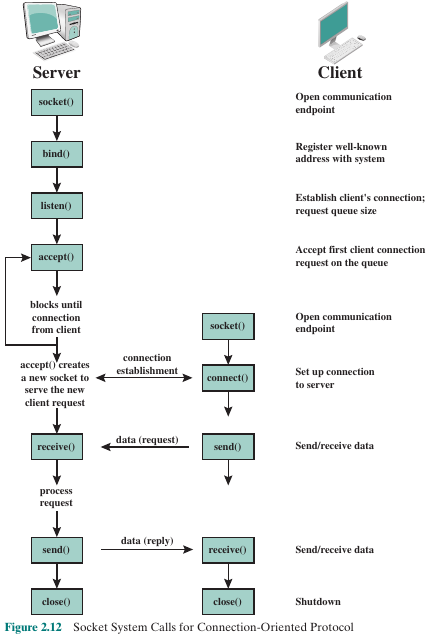
\includegraphics[height=0.8\textheight]{img/img17}
	\end{center}
\end{frame}

\begin{frame}
	\begin{center}
		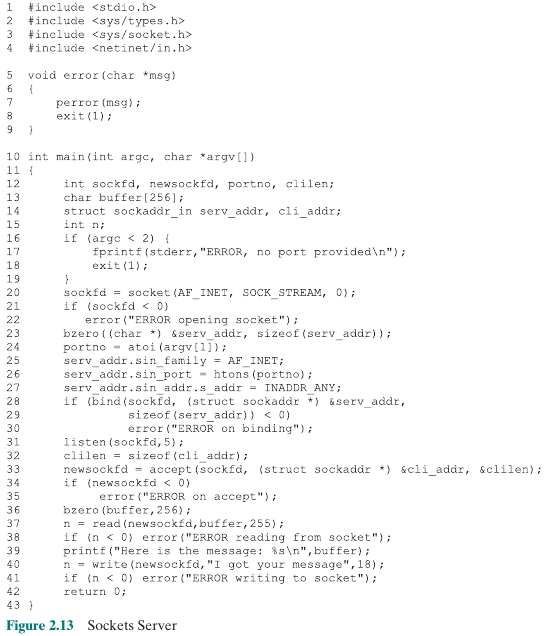
\includegraphics[height=0.9\textheight]{img/img18}
	\end{center}
\end{frame}

\begin{frame}
	\begin{center}
		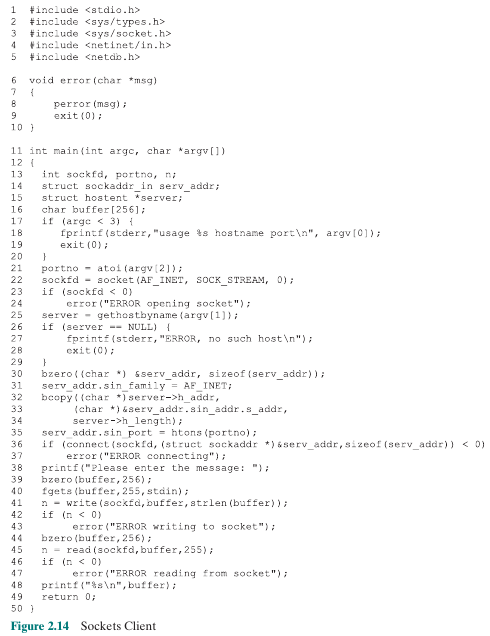
\includegraphics[height=0.9\textheight]{img/img19}
	\end{center}
\end{frame}

\begin{frame}
	\frametitle{Summary}
	\begin{itemize}
		\item The need for a protocol architecture
		\item Simple protocol architecture
		\item TCP/IP protocol architecture
		\begin{itemize}
			\item TCP/IP layers
			\item Operation of TCP and IP
			\item TCP and UDP
			\item IP and IPv6
			\item Protocol interfaces
		\end{itemize}
		\item Standardization within a protocol architecture
		\begin{itemize}
			\item Standards and protocol layers
			\item Service primitives and
			parameters
		\end{itemize}
	\end{itemize}
\end{frame}

\begin{frame}{Summary}
	\begin{itemize}
		\item Traditional internet-based applications
		\item Multimedia
		\begin{itemize}
			\item Media types
			\item Multimedia applications
			\item Multimedia technologies
		\end{itemize}
		\item Sockets programming
		\begin{itemize}
			\item The socket
			\item Sockets interface calls
		\end{itemize}
	\end{itemize}
\end{frame}

\begin{frame}
	\frametitle{Tugas Mandiri}
	\begin{itemize}
		\item Stallings, W. (2014). Data and Computer Communications, 10th Edition, New Jersey: Upper Saddle River\\
		\begin{itemize}
			\item Chapter 2 Protocol Architecture, TCP/IP, and Internet-Based Applications
		\end{itemize}
		\item Gupta, P. C. (2006). Data Communications and Computer Networks. New Delhi: Prentice Hall of India\\
		\begin{itemize}
			\item Section 6.8 Layered Architecture of the OSI Reference Model.
			\item Section 6.14.1 TCP/IP
		\end{itemize}
		\item Tanenbaum, A. S. \& Wetherall, D. J. (2013). Computer Networks, Fifth Edition. London: Pearson.\\
		\begin{itemize}
			\item Section 3.1 Protocol Hierarchies
		\end{itemize}
	\end{itemize}
\end{frame}

\begin{frame}
	\frametitle{Tugas Terstruktur}
	\textbf{Tampilkan Tugas 2}
\end{frame}

\end{document}
